\documentclass{article}

\usepackage{amsmath}
\usepackage{graphicx}
\usepackage{hyperref}

\usepackage[zihao=-4]{ctex}
\setCJKfamilyfont{hwzs}{STZhongsong}
\newcommand{\hwzs}{\CJKfamily{hwzs}}

\usepackage{geometry}
\geometry{
    a4paper,
    left=3cm,
    top=3cm,
    right=3cm,
    bottom=3cm
}

\usepackage{titlesec} % Tweak section
\titleformat*{\section}{\centering\bfseries\zihao{2}\hwzs}
\titleformat*{\subsection}{\zihao{-3}\heiti}
\titleformat*{\subsubsection}{\zihao{-4}\heiti}
\titlespacing*{\section}{0pt}{3\baselineskip}{2\baselineskip}
\titlespacing*{\subsection}{0pt}{\baselineskip}{\baselineskip}
\titlespacing*{\subsubsection}{0pt}{\baselineskip}{\baselineskip}

\usepackage{indentfirst}

% Centering pagenum
\usepackage{fancyhdr} 
\fancypagestyle{plain}{%
    \fancyhf{}
    \fancyfoot[C]{\zihao{-5}\thepage}
    \renewcommand{\headrulewidth}{0pt}
}
\pagestyle{plain} 

% Para space
\usepackage{setspace}
\renewcommand{\baselinestretch}{1.5}

\usepackage{caption}
\captionsetup{
    margin=0.5ex,
    font={small,bf}
}

% Code display
\usepackage{xcolor}
\definecolor{lbcolor}{rgb}{0.98,0.98,0.98} 
\usepackage{listings}
\lstset{
    basicstyle=\ttfamily,
    breaklines=true,
    backgroundcolor=\color{lbcolor},
    postbreak=\mbox{\textcolor{red}{$\hookrightarrow$}\space}
}


% Table font
\let\oldtable\table
\let\oldendtable\endtable
\def\table[#1]{\oldtable[#1]\zihao{5}}
\def\endtable{\oldendtable}

% Crossref
\usepackage{cleveref}
\crefformat{equation}{式~(#2#1#3)}
\crefformat{table}{表~#2#1#3}
\crefformat{figure}{图~#2#1#3}

% Booktabs
\usepackage{booktabs}

% TOC tweak
\usepackage{tocloft}
\renewcommand{\cfttoctitlefont}{\vspace{3\baselineskip}\hfill\centering\bfseries\zihao{2}\hwzs}
\renewcommand{\cftaftertoctitle}{\hfill\vspace{2\baselineskip}}
\renewcommand{\cftsecfont}{\bfseries\zihao{-4}\songti}
\renewcommand{\cftsubsecfont}{\zihao{-4}\songti}


\def\keywords#1{\noindent\textbf{关键词:#1}}
\def\keywordsEn#1{\noindent\textbf{Keywords: #1}}
\def\abstractZH{
    \zihao{-4}
    {\centering\bfseries\zihao{2}摘要\par\vspace{1ex}}
}
\def\endabstract{}
\def\abstractEN{
    \zihao{-4}
    {\centering\bfseries\zihao{2}Abstract\par\vspace{1ex}}
}
\def\endabstract{}

% Variable
\def\NUM{\mathrm{NUM}}
\def\COST{\mathrm{COST}}
\def\GDP{\mathrm{GDP}}

\title{基于VAR模型的我国旅游经济研究}
\date{}

\begin{document}
    \maketitle    

    \begin{abstractZH}
        随着国民收入的提高,人们的物质文化需求不断增长,外出旅游成为
        许多人的选择。
        本文利用VAR模型,建立GDP、旅游成本以及旅游需求之间的联系,
        并通过脉冲响应函数和方差分解等技术分析得到相互之间的动态影响,
        给出了一些与发展旅游市场经济相关的参考意见。

        \keywords{时间序列;VAR模型;脉冲响应函数;方差分解;旅游}

    \end{abstractZH}

    \newpage
    \setcounter{page}{1}
    \begin{abstractEN}
        With the increasing of national income, 
        material and cultural needs of the public
        continue to grow. And traveling is becoming one
        of the main entertainment choices.
        This paper bridges a relationship among GDP, tourism cost and
        demand via VAR model. And with the help of impulse response
        and forecast error variance decomposition (FEVD), some
        reference advices of tourism market development are provided.

        \keywordsEn{time series analysis; VAR; FEVD; IRF; tourism}
    \end{abstractEN}


    \newpage
    \tableofcontents

    \newpage
    \setcounter{page}{1}
    \section{引言}
    随着国民经济收入的不断增长,人们的物质文化需求逐渐提升,
    旅游作为一种文化消遣方式的重要性逐渐提升,越来越多的人们
    利用假期甚至是周末的休闲时光出门旅游,旅游业的迅速增长
    促进了我国经济的发展,而反过来人们收入水平的提高亦会
    增长人们的旅游需求。

    \section{文献综述}
    随着旅游业成为学术界研究的一个热点领域,各种各样的
    模型和理论被运用其中,比较常见的有VAR、ECM、TVP等计量模型,
    这大大促进了领域专业性的发展\cite{song2006forecasting}。
    许多学者会利用VAR以及脉冲响应和方差分解分析的方式
    进行建模,
    余丹阳\cite{余丹阳2018基于}选取了湖南省的旅游数据,
    构建VAR模型,并对其进行脉冲响应分析和方差分解分析,
    研究了湖南省旅游总收入与湖南省GDP的相互影响关系;
    王纯阳\cite{王纯阳2010基于}
    利用美国客源市场的相关数据,
    建立旅游需求与旅游价格、收入、替代价格等变量之间的
    VAR模型发现美国对中国的旅游需求
    受到自身的波动、旅游价格等影响;
    吴丽云\cite{吴丽云2010我国旅游业与经济增长的关系分析}
    采用协整性检验和Granger因果检验方法对我国1985年以来的
    国内旅游、入境旅游、出境旅游和经济增长之间的关系进行了检验,
    发现经济增长与国内旅游业的发展相辅相成,
    但出境旅游对中国经济增长有一定的抑制作用。

    总的说来,国内学者们利用一些计量模型,探讨了旅游要素和
    我国经济要素的之间的一些相关关系,本文从向量自回归模型(VAR)
    入手,建立旅游需求、成本和我国经济水平的相关关系,
    同时利用脉冲响应函数与方差分解等技术探讨在各个变量的
    冲击下,各个变量的相应的动态影响,探讨了我国旅游经济市场的
    一些均衡规律,希望对我国相关旅游经济政策的指定和有关部门法规法则
    的颁布实施提供一个较为科学的参考。

    \section{变量选取与数据来源}
    我们从中国统计年鉴\cite{中华2014中}中选取了1994年至2019年的我国人均GDP、
    国内旅游人次以及人均旅游花费,并进行对数变换,分别记为$\GDP,\NUM,\COST$:
    \begin{enumerate}
        \item 人均GDP。人均GDP能衡量人们的生活水准,从而很大程度上对于
        旅游行为有着重要的影响,从而我们选取其作为我们最后一个
        内生变量。

        \item 国内旅游人次。在许多研究中,常常使用旅游人数来衡量
        旅游需求,另一个比较常用的变量是旅游支出\cite{witt1995forecasting}。
        本文采用国内的旅游人次作为内生变量之一。

        \item 人均旅游花费。旅游花费可以衡量旅游成本,从另一侧面
        也能表现旅游需求,我们也将其作为我们的内生变量之一。
    \end{enumerate}

    \section{模型选取与实证分析}
    \subsection{模型设定}
    VAR模型是把系统中每一个内生变量看作系统中内生变量的
    滞后值的函数,是一维的AR模型的向量版,对于我们的VAR($p$)模型来讲,
    其表达式为
    \[X_t=\beta_0+\beta_1X_{t-1}+\cdots+\beta_2X_{t-p}+u_t\]
    这里$X_t=(\NUM_t,\COST_t,\GDP_t)^\mathrm T$,$\beta_0$为3维向量,
    而$\beta_i,i=1,\ldots,p$为$3\times 3$矩阵。

    首先我们需要确定模型的最优滞后阶数,各种信息准则(\cref{tab:AIC BIC})
    的最优滞后阶数
    在6、7阶左右,但是太长的滞后阶数会增加模型的复杂度,本着简单为上
    的原则,我们注意到滞后阶数1在一个局部范围内是较优的,从而我们选择
    滞后阶数为1。

    \begin{table}[h]
        \caption{不同滞后阶数下的信息准则}
        \label{tab:AIC BIC}
        \centering
        \begin{tabular}{lrrrr}
            \toprule
            滞后阶数 & AIC &       BIC&        FPE &       HQIC \\
            \midrule
            0 &    -11.87 &    -11.73 & 6.967e-06 &    -11.86 \\
            1 &    -21.14 &    -20.55 & 6.767e-10 &    -21.08 \\
            2 &    -20.80 &    -19.77 & 1.083e-09 &    -20.70 \\
            3 &    -22.82 &    -21.35 & 2.060e-10 &    -22.68 \\
            4 &    -25.96 &    -24.05 & 2.280e-11 &    -25.77 \\
            5 &    -102.9 &    -100.5 & 2.654e-43 &    -102.6 \\
            6 &    -192.7 &    -189.9 &-1.438e-83*&     -192.4 \\
            7 &   -194.2* &   -191.0* &-9.104e-86 &   -193.9* \\
            8 &    -192.6 &    -188.9 &-4.709e-86 &    -192.3 \\
            9 &    -193.9 &    -189.7 &-2.260e-87 &    -193.4 \\
            \bottomrule
        \end{tabular}
    \end{table}

    选取最优滞后阶数为1后,我们得到估计值
    \[\hat\beta_0=\begin{pmatrix}
        -0.068696 \\
        0.735973  \\
        0.478064
    \end{pmatrix},
    \hat\beta_1=\begin{pmatrix}
        0.778315 & -0.150901 & 0.279133\\
        -0.052785 & 0.670381 & 0.180302\\
        -0.104600 & -0.223922 & 1.18356
    \end{pmatrix}\]

    \subsection{平稳性检验}
    为避免出现伪回归现象所导致的无效分析,
    再进一步的检验前,我们需要验证模型中的序列是平稳的。
    但从趋势图(\cref{fig:data trend})中明显可以看出是不平稳的,
    相应的ADF检验(\cref{tab:data adf})也得出了一致的结论。
    \begin{table}[h]
        \zihao{5}
        \caption{数据的ADF检验}
        \label{tab:data adf}
        \centering
        \begin{tabular}{lrrr}
            \toprule
            变量 & 统计量 & p值 & 滞后阶数 \\
            \midrule
            $\NUM$  & -1.303 & 0.628 & 7 \\
            $\COST$ & -1.358 & 0.602 & 9 \\
            $\GDP$  & -2.001 & 0.286 & 9 \\
            \bottomrule
        \end{tabular}
    \end{table}

    \begin{figure}[h]
        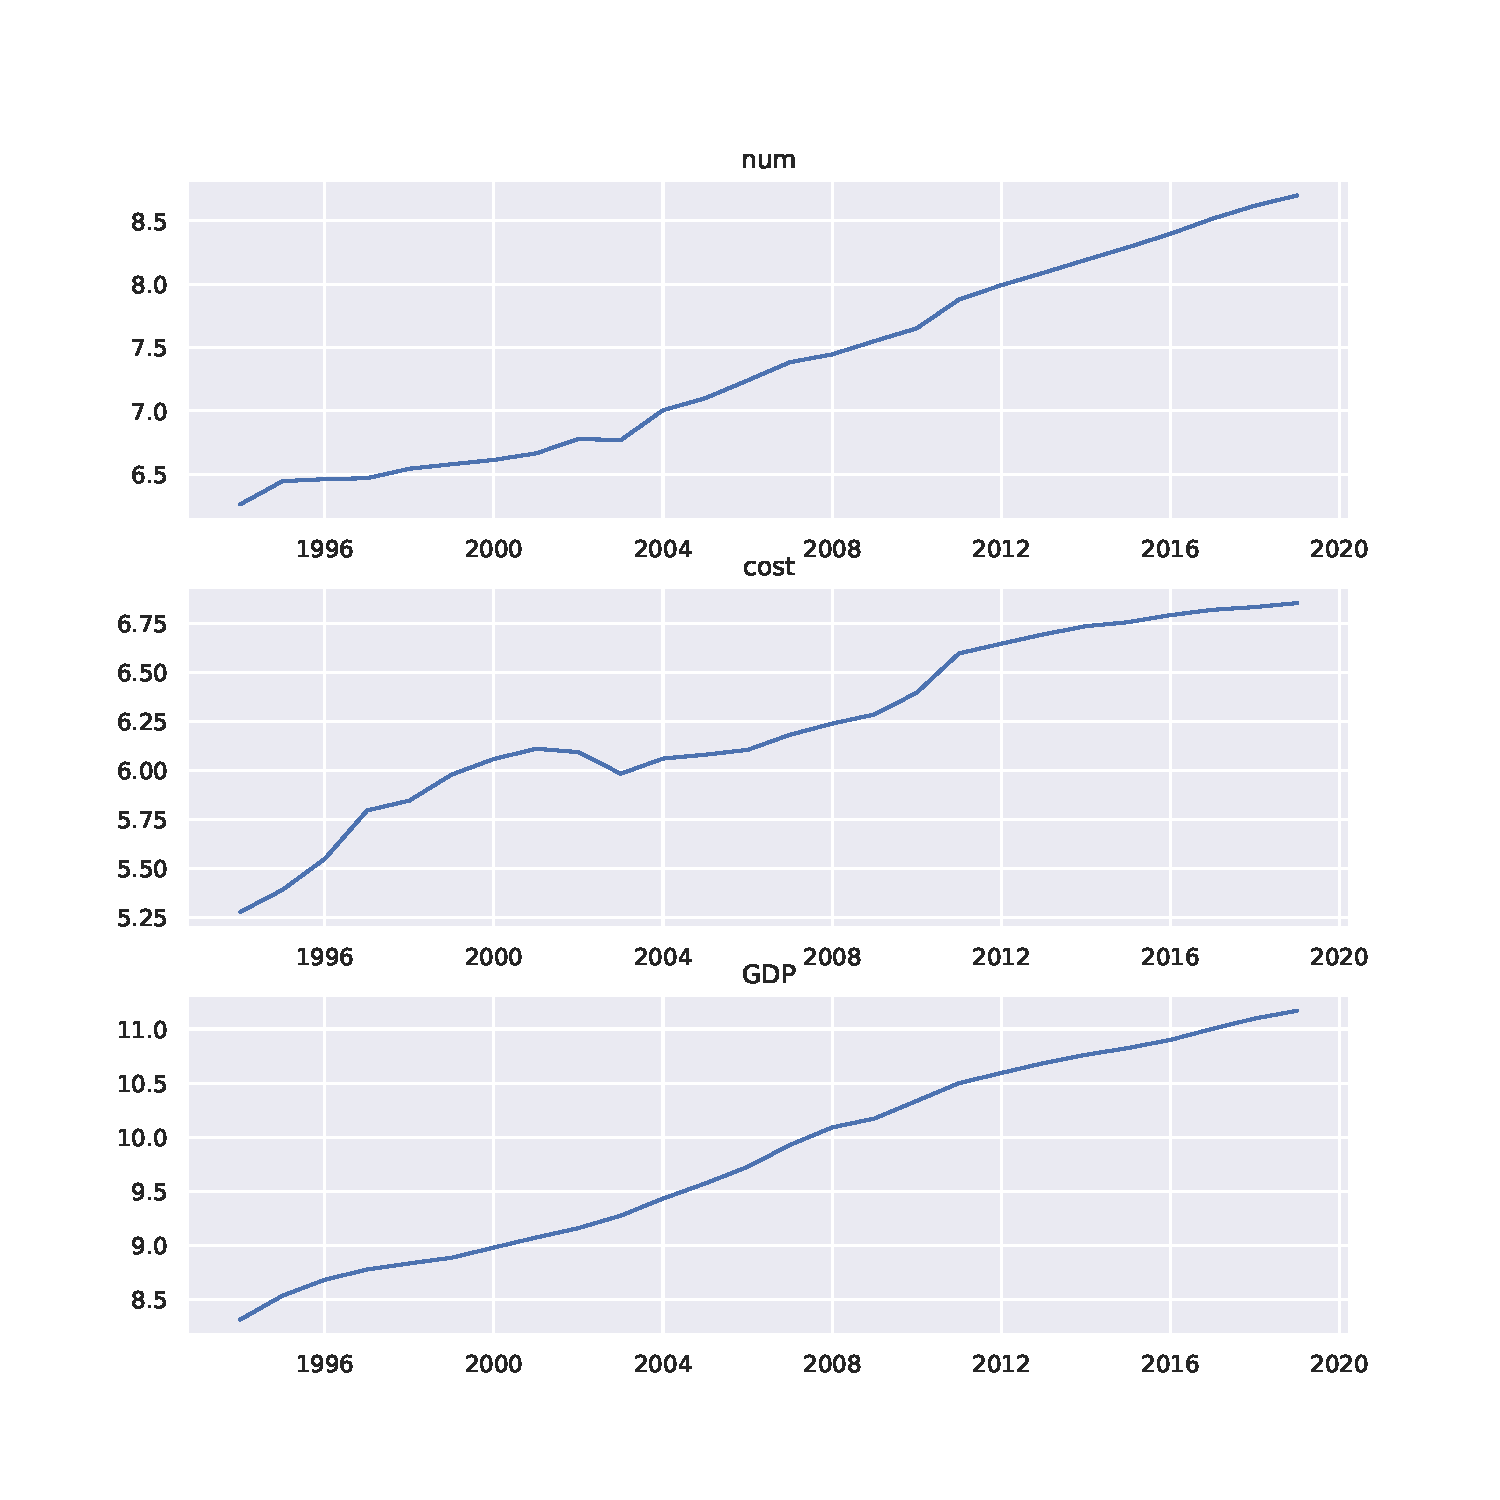
\includegraphics[width=\textwidth]{trend}
        \caption{数据趋势图}
        \label{fig:data trend}
    \end{figure}

    我们可以考虑数据的一阶差分,进行ADF检验(\cref{tab:delta data adf})
    可以发现,仅有国内旅游总人次($\NUM$)
    的差分是是平稳的,而另外两个数据的差分仍然不平稳。
    同时注意到差分会损失数据量,这对于本文中本来数据量就不多情况是一个比较
    大的影响。
    \begin{table}[h]
        \caption{一阶差分的ADF检验}
        \label{tab:delta data adf}
        \centering
        \begin{tabular}{lrrr}
            \toprule
            变量 & 统计量 & p值 & 滞后阶数 \\
            \midrule
            $\Delta\NUM$  & -5.144 & 0.000 & 0 \\
            $\Delta\COST$ & -2.569 & 0.100 & 9 \\
            $\Delta\GDP$  & -1.924 & 0.321 & 8 \\
            \bottomrule
        \end{tabular}
    \end{table}

    \subsection{协整检验}
    我们尝试对这三个变量进行协整检验。
    协整指多个非平稳变量的某种线性组合是平稳的,这样这个
    线性组合可以描述原来变量的均衡关系。
    这里我们采用协整关系表达式为
    \[\GDP = \beta_1\COST + \beta_2\NUM + u_t\]
    进行简单的基于回归残差的协整检验。
    首先进行OLS回归可以得到相应估计值$\hat\beta_1=0.5870,\hat\beta_2=0.8353$
    均显著,而对残差进行ADF检验可以知残差为平稳的。
    从而我们可以知道,三个内生变量之间具有长期的均衡关系,
    这保证了之后所进行的Granger因果检验以及脉冲相应等VAR分析是有意义的。
    同时也表明了人均消费和旅游人数对人均GDP的促进作用。
    \begin{table}[h]
        \caption{残差的ADF检验}
        \label{tab:resid adf}
        \centering
        \begin{tabular}{lrrr}
            \toprule
            统计量 & p值 & 滞后阶数 \\
            \midrule
            -7.052 & 0.000 & 8 \\
            \bottomrule
        \end{tabular}
    \end{table}
    
    \subsection{Granger因果检验}
    协整检验结果表明变量之间是否存在长期的均衡关系,
    但是这种关系是否构成因果关系还需要进一步验证。
    格兰杰因果关系检验的基本观念在于:未来的事件不会对目前与过去产生因果影响,
    而过去的事件才可能对现在及未来产生影响\cite{granger1969investigating,seth2007granger}。
    也就是说,对于时间序列变量$X$和$Y$,如果$X$是$Y$变化的原因,
    则$X$的变化应该发生在$Y$变化之前,而且$X$的过去值应该有助于预测$Y$的未来值,
    但$Y$的未来值不应该能预测$X$的未来值\cite{庞皓2019计量经济学}。

    我们对三个内生变量做Granger因果检验的结果如\cref{tab:granger}所示,
    可以发现,人均GDP是旅游人数的Granger原因,人均消费是人均GDP的Granger原因。
    不过需要注意到的是
    Granger因果关系检验的结论只是一种统计估计,不是真正意义上的因果关系,
    不能作为肯定或否定因果关系的根据。

    \begin{table}[h]
        \caption{Granger因果检验结果}
        \label{tab:granger}
        \centering
        \begin{tabular}{lrrc}
            \toprule
            原假设 & F统计量 & p值 & 结论 \\
            \midrule
            $\COST$不能Granger引起$\NUM$ & 2.707  & 0.105 & 不拒绝 \\
            $\GDP$不能Granger引起$\NUM$  & 5.761  & 0.019 & 拒绝 \\
            $\NUM$不能Granger引起$\COST$ & 0.1876 & 0.666 & 不拒绝 \\
            $\GDP$不能Granger引起$\COST$ & 2.198  & 0.143 & 不拒绝 \\
            $\NUM$不能Granger引起$\GDP$  & 1.851  & 0.178 & 不拒绝 \\
            $\COST$不能Granger引起$\GDP$ & 13.69  & 0.000 & 拒绝 \\
            \bottomrule
        \end{tabular}
    \end{table}

    \subsection{脉冲响应函数分析}
    脉冲响应函数描述一个内生变量对误差冲击的反应,即在随机误差项上
    施加一个标准差大小的冲击后对内生变量的当期值和未来值所带来的影响,
    刻画了变量之间动态交互作用。

    在进行脉冲响应分析前,我们对VAR的平稳性进行检验,否则脉冲响应分析将可能是无效的。
    对于我们建立的VAR模型,能得到其特征值为0.98, 0.88, 0.77,全部在单位圆之内,故模型
    是平稳的。从而下面给出三个变量之间脉冲响应函数的图像(\cref{fig:irf})。
    横轴代表作用的滞后期数(年),纵轴表示变化程度。实线为脉冲响应函数,虚线为
    正负二倍标准差偏离带。

    从\cref{fig:irf}第一排
    可以看出,在本期给旅游人数一个正的冲击,
    人数增加很大,但随着滞后阶数的增加,正效应逐渐转化为负效应,
    但程度没有之前大。其主要原因可能是因为国内旅游体验质量并不太高,
    导致游客忠诚度较小。
    同时可以看到,人均旅游花费会给旅游人次带来负的效应,
    尽管在当期没有影响,但随着滞后期数
    的增加,影响逐渐平稳。
    人均GDP的正向冲击虽然在当期没有影响到旅游人次,
    但随着滞后期数的增加,旅游人次受到的正向冲击逐渐增大,并趋于一个稳定值。

    对于旅游人均消费来说,自己的正向冲击在初期会带来正的影响,但影响随后迅速
    下降至负的,随后趋于稳定;而旅游人数的正向冲击在当期没有影响,
    但后面会表现为负的影响,直到趋于一个较稳定的值;人均GDP的正向冲击
    在当期亦没有影响,但随后表现为正的影响,并迅速上升,大约在10期达到
    峰值,随后逐渐下降。即人均GDP还是能比较大地增加消费水平,而旅游人数
    总体上表现为一个相对人均GDP较小的负的影响。

    从最后一排可以看到,对于人均GDP来讲,自己对自己的正向冲击是有正向影响的,
    且在当期就会表现出来,同样也是在10期达到峰值,随后缓慢下降;而旅游人次
    与人均消费带来的都是后续的负效应。对于旅游人次来说,负效应缓慢增加并趋于
    稳定,而消费水平的负效应则是在10期达到峰值,后面稍有减弱。

    \begin{figure}[h]
        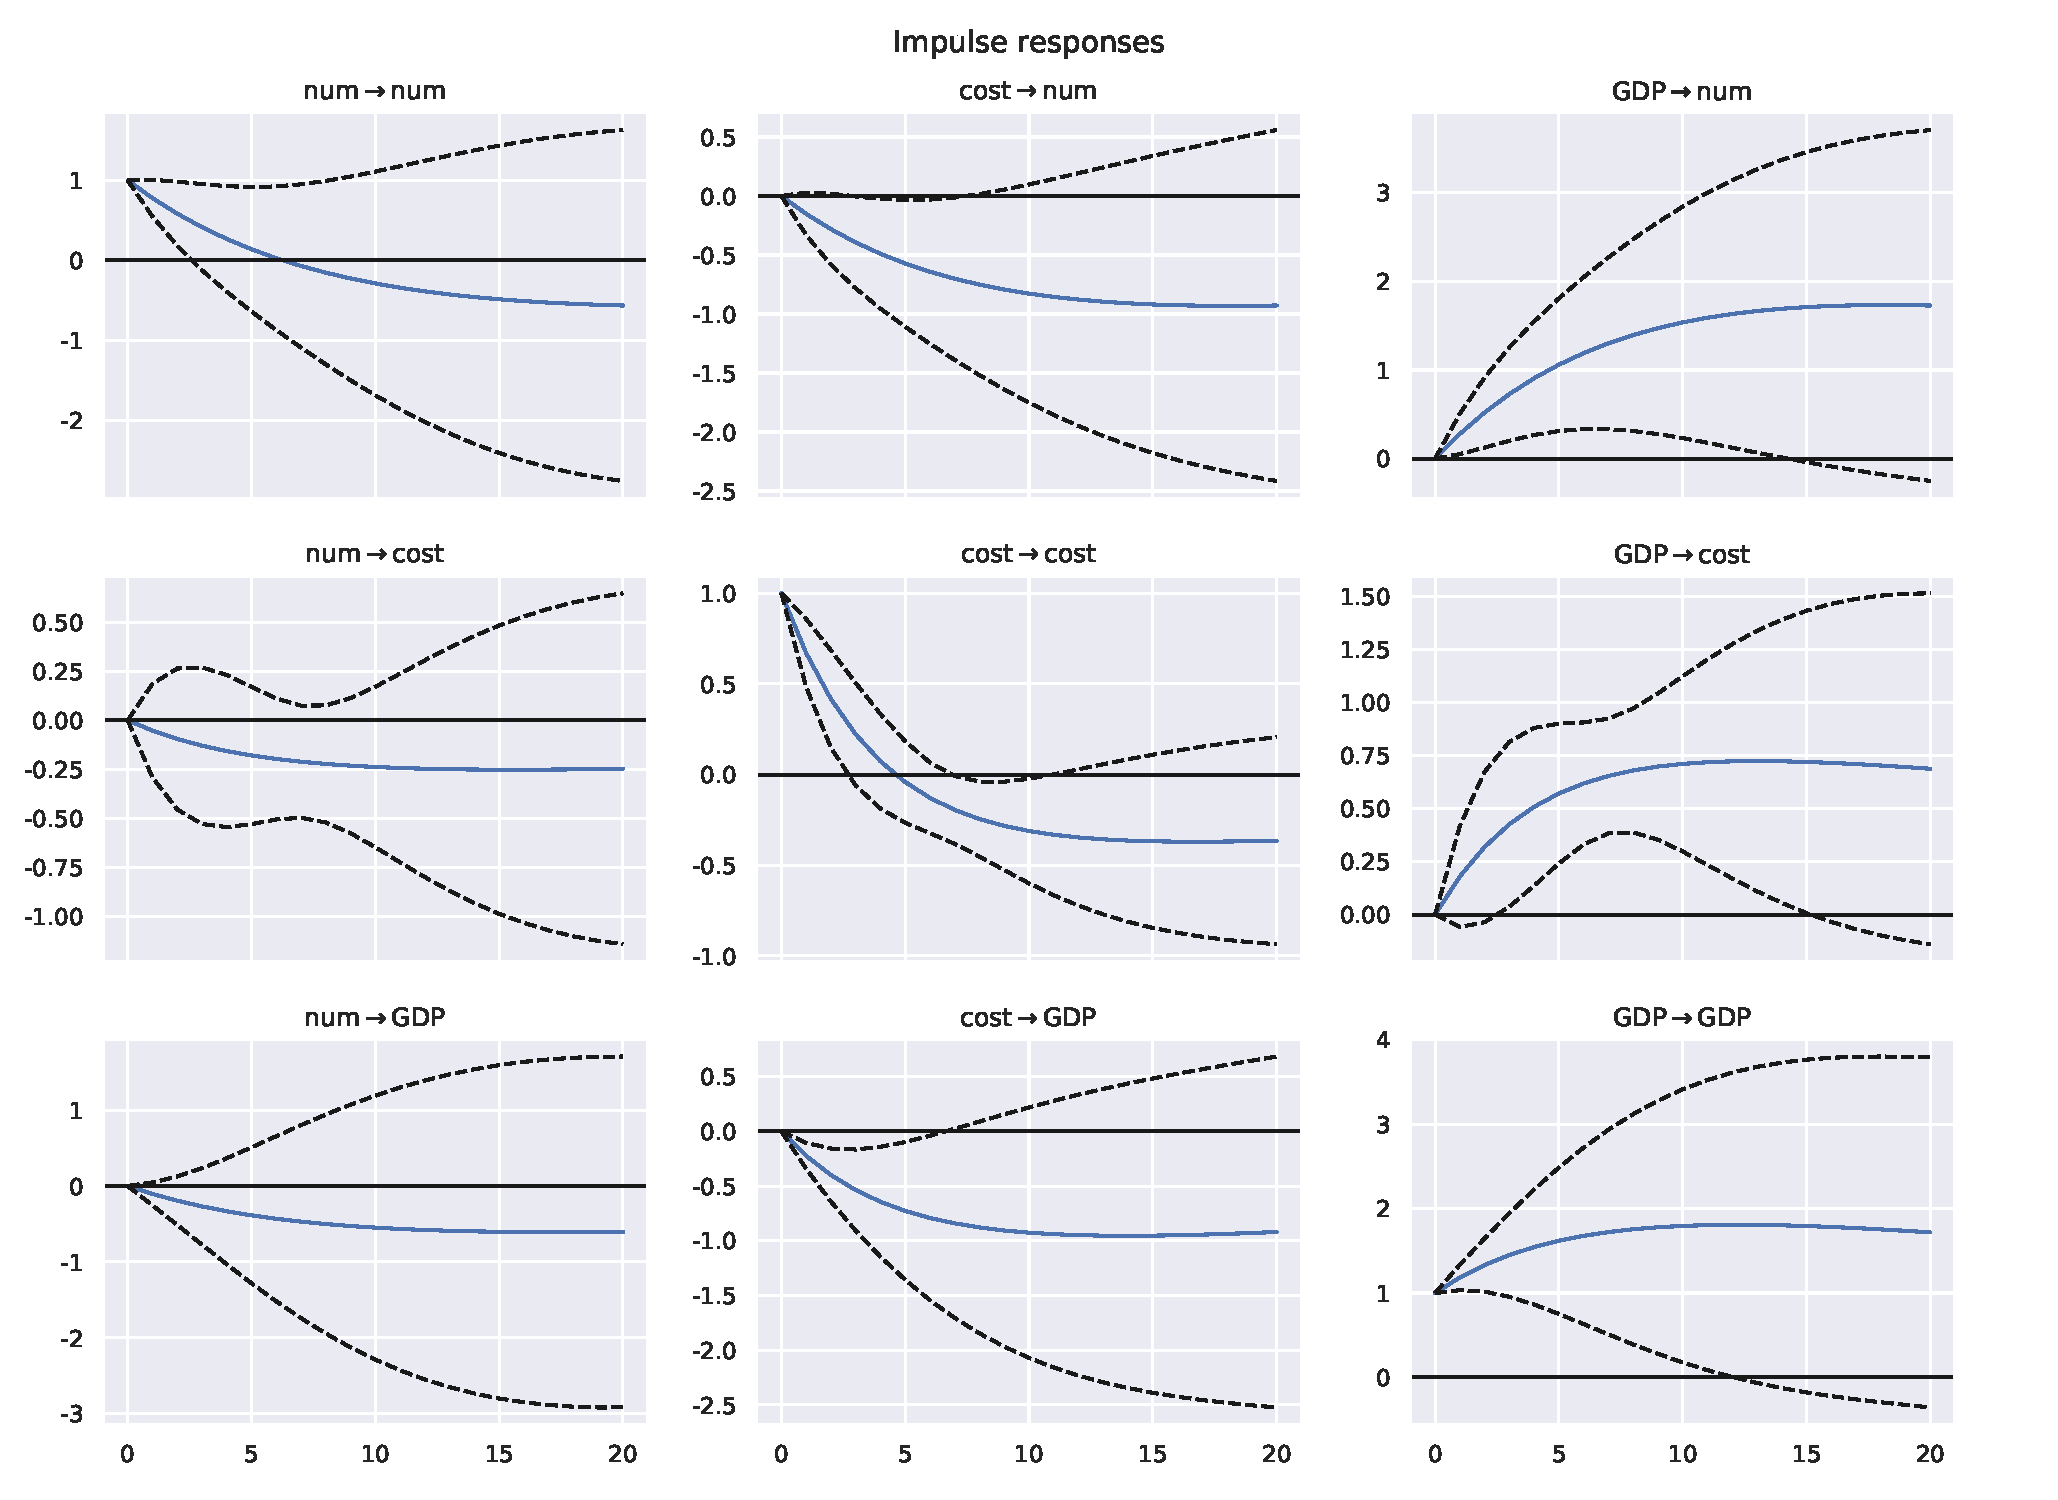
\includegraphics[width=\textwidth]{irf}
        \caption{脉冲响应函数}
        \label{fig:irf}
    \end{figure}

    \subsection{方差分解}
    方差分解是另一种评价VAR模型的方法,它能给出随机信息的
    相对重要性,预测误差的特征,从而揭示系统中各个变量的相互关系。
    预测误差的方差分解时序列中由于其自身的冲击与其他变量的冲击而导致的
    变动的比例。

    我们对每个内生变量的方差如\cref{fig:fevd}所示。可以看到
    在最开始时,旅游人次冲击对自身的贡献程度最大,但随着时间推移,
    贡献程度逐渐下降至10\%左右,而人均GDP和人均消费逐渐占据主要贡献,
    分别到达30\%和60\%。即受人均消费影响最大,人均GDP其次。

    而对于人均消费来说,基本上由自身贡献了较大的影响,虽然随着时间推移
    有着缓慢的下降,但基本上能保持在68\%以上的贡献,剩下的贡献几乎由
    人均GDP提供,而不受旅游人次的影响。也就是说,人均消费基本上不受旅游人次的
    影响。

    对于人均GDP来说,最开始时自身占据主要影响,达到67\%左右,而之后
    自身影响逐渐下降,趋于30\%左右;人均消费占据的影响逐渐上升,
    达到60\%左右;而旅游人数仅在初期有明显的影响,到后面基本上没有影响。

    \begin{figure}[h]
        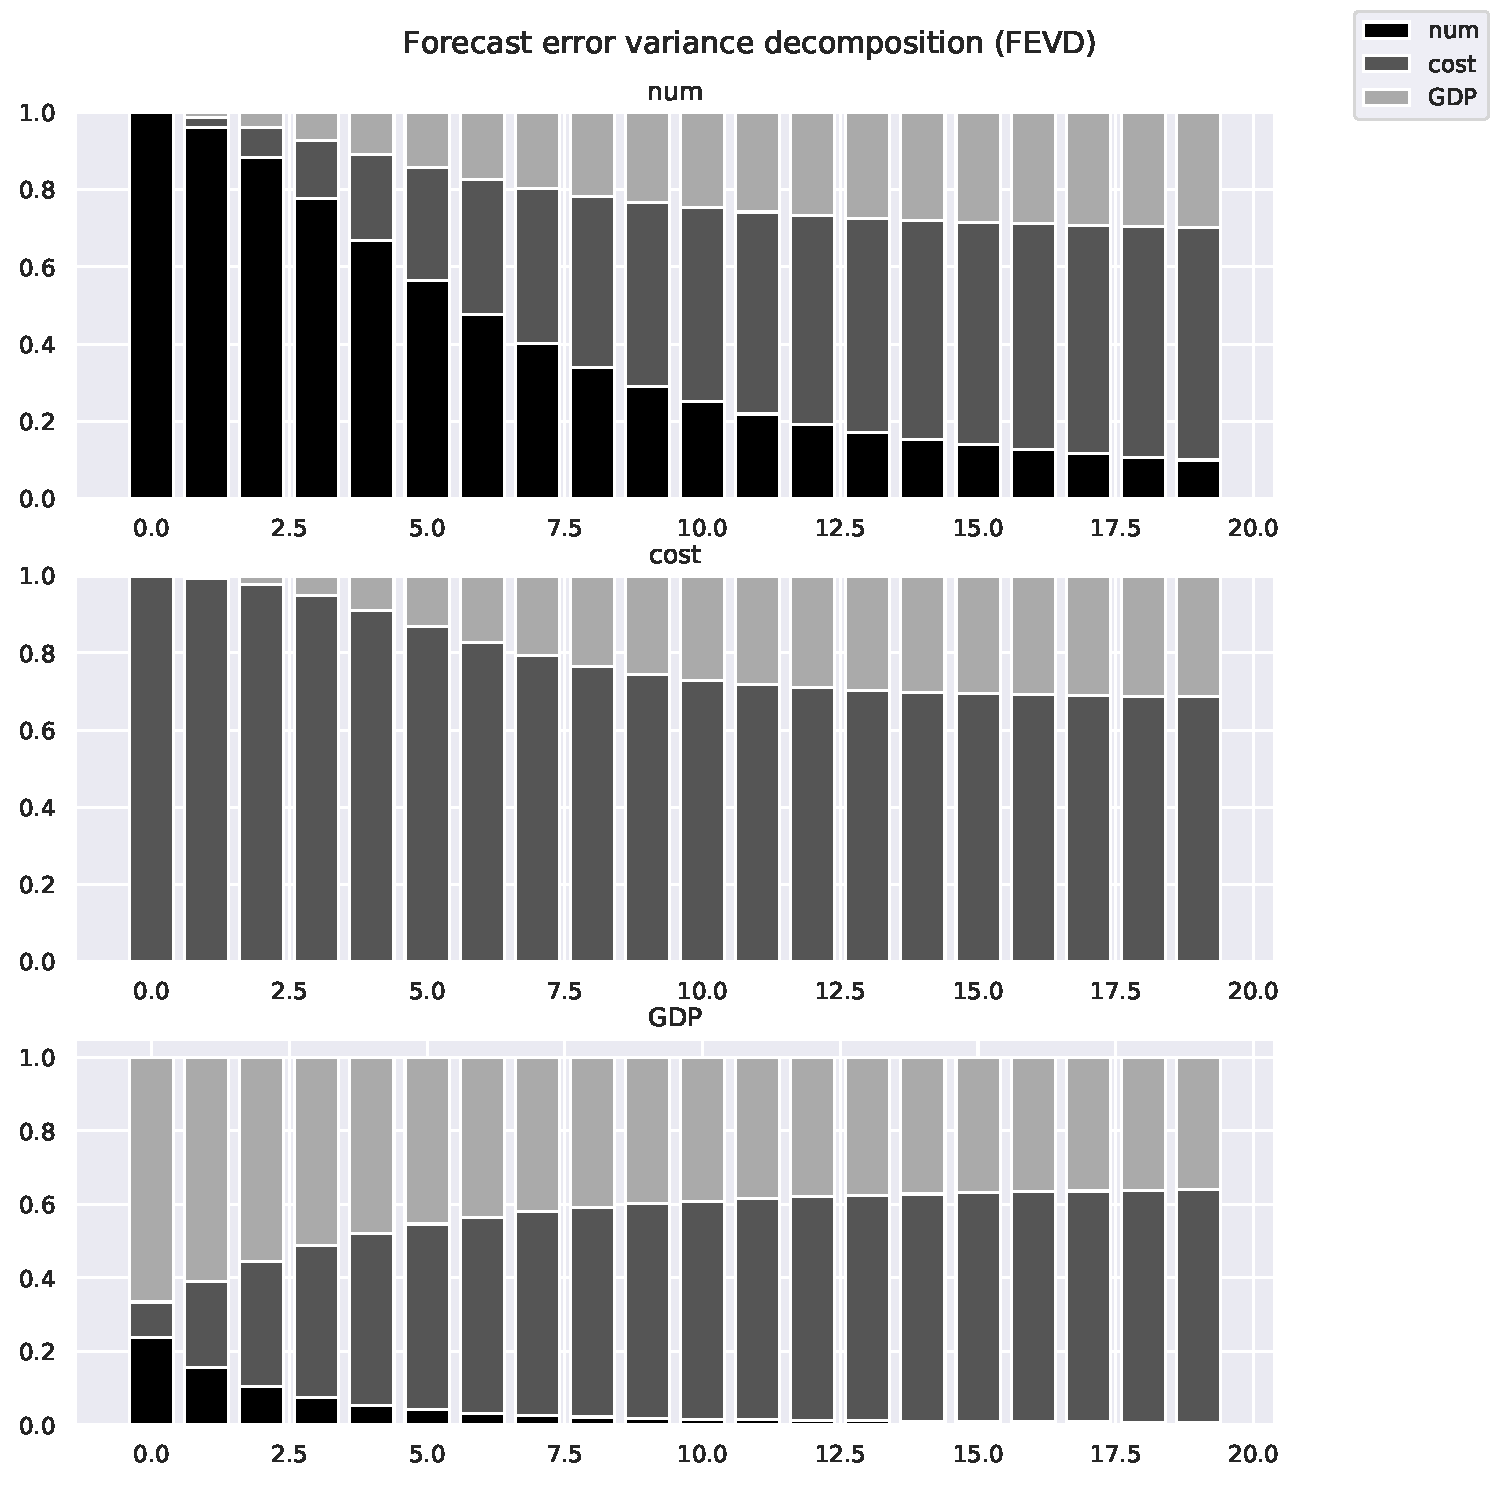
\includegraphics[width=\textwidth]{FEVD}
        \caption{方差分解}
        \label{fig:fevd}
    \end{figure}
    
    \section{研究结论}
    综合前面的分析结果,我们可以得到一系列的与国内旅游经济相关的结论。

    \begin{enumerate}
        \item
        旅游需求(旅游人次)主要受人均GDP与人均消费的影响较大。对于较高的
        人均GDP与较低的人均消费,旅游人次会有一个明显的增加。而消费的影响是当期就
        比较明显的,所以为了提升国内的旅游需求,各个旅游景点不妨出台一些相关的优惠政策
        来吸引游客,应该会有比较显著的效果。

        \item

        考虑到旅游人次对自身的冲击属于先正后负,可能是由于旅游质量不高所引起的,
        较少的游客会有二次游览的现象。例如频发的景区商贩坐地起价,黑导游、不合理低价团等等,
        以及景区拥堵、景区垃圾等一些一直困扰公众的问题。利益的驱使使部分景区商家、
        旅行社失去底线,有关部门应加大监管力度,切实保护消费者的合法权益,
        相应的违法行为应依法惩处。同时对于景区拥堵这一现象,建议国家相关部门落实
        带薪休假制度,可以适当错峰休假,这样可以在很大层面上缓解热点景区在
        节假日“人山人海”的拥堵状况,也从一定程度上避免了由于需求过于旺盛,
        商家得以借机乱定价、定高价的行为。
    \end{enumerate}

    通过向量自回归模型,我们分析了人均GDP、人均旅游消费以及旅游人数三者的关系,
    了解了国内旅游市场的一些需求规律,这对促进我国旅游经济发展和相关政策
    的制定是一个比较重要的参考意见。同时也应该指出的是,由于本文的中考虑的内生
    变量较少,没有考虑到一些比较重要的如国际旅游形势、季节趋势等影响,
    而且样本量也不是很大,可能存在一部分的小样本偏差,这两方面仍然有很大的改进空间。

    \bibliographystyle{unsrt}
    \bibliography{refs}

    \newpage
    \section{致谢}
    感谢老师一学期的辛勤付出,虽然由于时局特殊,大家见面的机会不多,
    但是仍旧是充实而厚重的一学期。同时感谢那些对我提供学习上的
    帮助的同学,没有他们的帮助,这篇论文也无法及时完成。

    \newpage
    \appendix
    \section{代码(Python)}
    \lstinputlisting[language=Python]{var.py}
\end{document}